\documentclass{article}

\usepackage[portuguese]{babel}

\usepackage{amsmath, amssymb}
\usepackage{graphicx}
\usepackage[colorlinks=true, allcolors=blue]{hyperref}

\usepackage[section]{placeins}

\title{Relatório 01}
\author{Vinícius de Oliveira Peixoto Rodrigues (245294)}
\date{Agosto de 2022}

\begin{document}
\maketitle

\section*{Questão 1}

\begin{figure}[!ht]
    \begin{center}
        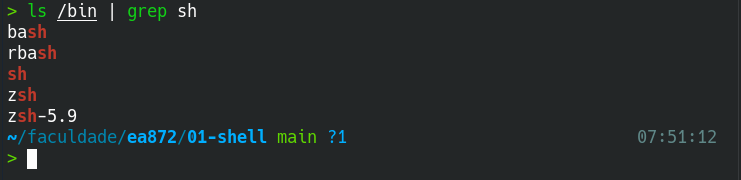
\includegraphics[width=\textwidth]{images/q1.png}
        \caption{Lista de \textit{shells} instaladas no sistema}
    \end{center}
\end{figure}

As \textit{shells} no meu sistema são instaladas pelo \textit{package manager} em \texttt{/bin}, de modo que um \texttt{grep} é o suficiente para encontrar as \textit{shells} instaladas. A minha distribuição vem por padrão com \texttt{bash} e \texttt{sh}, e o \texttt{zsh} foi instalado por mim.

\FloatBarrier


\newpage
\section*{Questão 2}

\begin{figure}[!ht]
    \begin{center}
        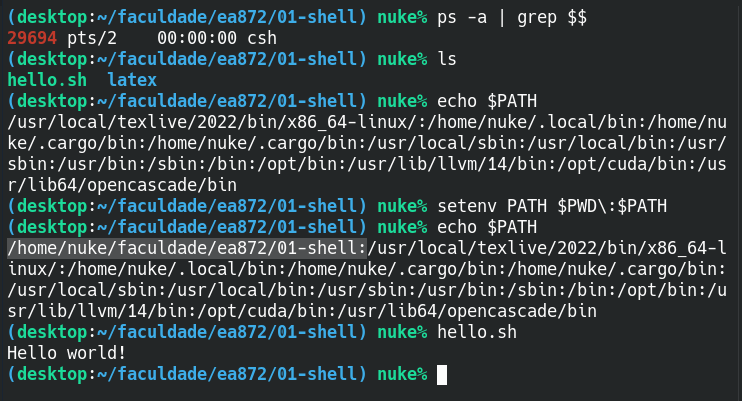
\includegraphics[width=\textwidth]{images/q2.png}
        \caption{Adicionando um novo caminho ao \texttt{\$PATH} do \texttt{csh}}
        \label{fig:q2}
    \end{center}
\end{figure}

Para modificar uma \textit{environment variable} no \texttt{csh}, utiliza-se o comando

\begin{center}
    \texttt{setenv <var> <value>}
\end{center}

A Figura \ref*{fig:q2}
ilustra esse processo adicionando um script \texttt{hello.sh} no diretório local, concatenando em seguida o \texttt{\$PWD} ao \texttt{\$PATH} da \textit{shell}.

\FloatBarrier

\section*{Questão 3}

A tabela abaixo contém os valores, assim como uma explicação breve sobre cada um deles:

\begin{center}
    \begin{tabular}{|c|c|c|}
        \hline
        \textbf{Variável} & \textbf{Valor} & \textbf{Explicação} \\
        \hline
        \texttt{\$0} & prog & nome do arquivo \\
        \hline
        \texttt{\$2} & le-27 & segundo argumento \\
        \hline
        \texttt{\$4} & unicamp & quarto argumento \\
        \hline
        \texttt{\$8} & brasil & oitavo argumento \\
        \hline
        \texttt{\$\$} & <número> & \texttt{pid} da \textit{shell} \\
        \hline
        \texttt{\$\#} & 11 & numero de argumentos \\
        \hline
        \texttt{\$*} & prog le-27 feec unicamp campinas são paulo... & concatenação dos argumentos \\
        \hline
        \texttt{\$@} & prog le-27 feec unicamp campinas são paulo... & lista dos argumentos \\
        \hline
        
    \end{tabular}
\end{center}

\section*{Questão 5}


\begin{figure}[!ht]
    \begin{center}
        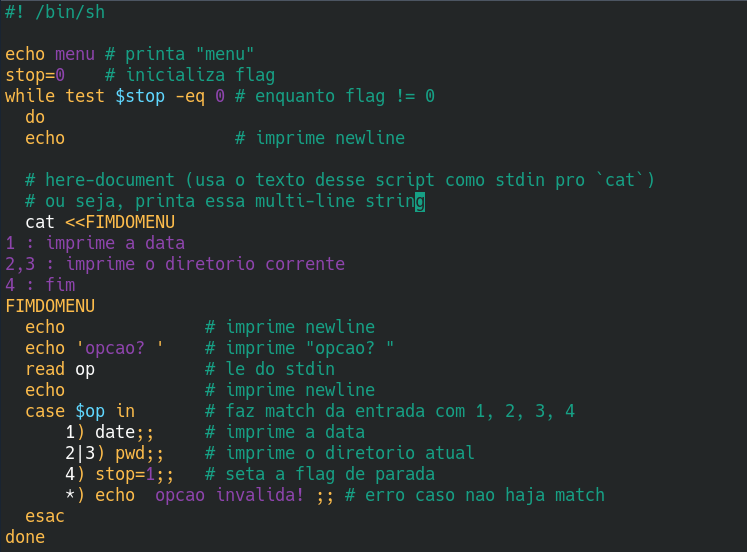
\includegraphics[width=\textwidth]{images/q5_a.png}
        \caption{Item (a)}
    \end{center}
\end{figure}

\begin{figure}[!ht]
    \begin{center}
        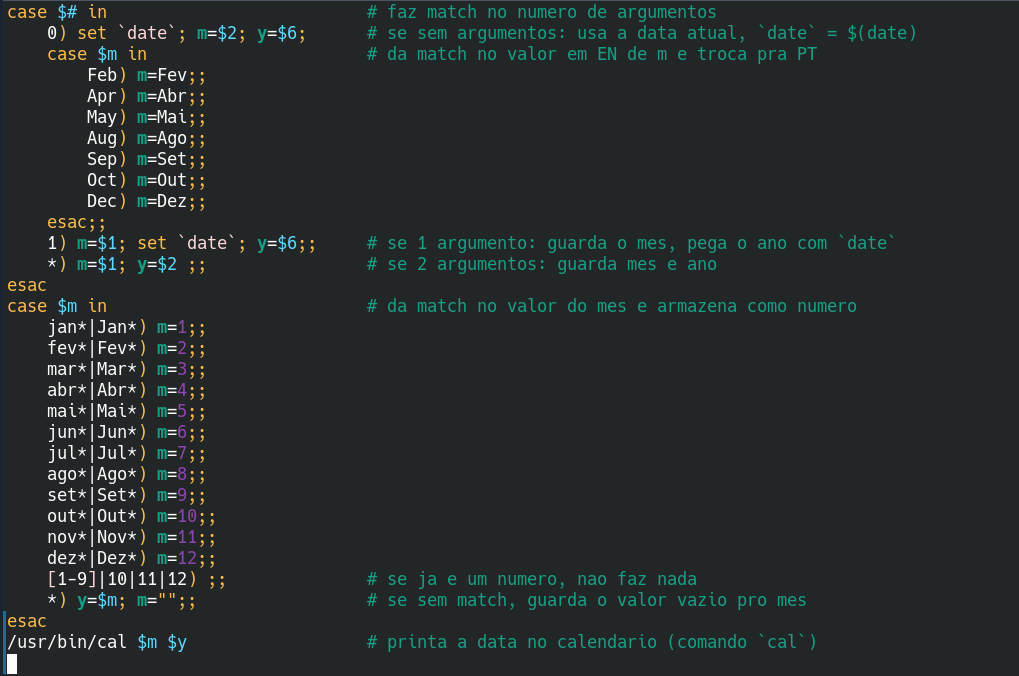
\includegraphics[width=\textwidth]{images/q5_b.png}
        \caption{Item (b)}
    \end{center}
\end{figure}

\begin{figure}[!ht]
    \begin{center}
        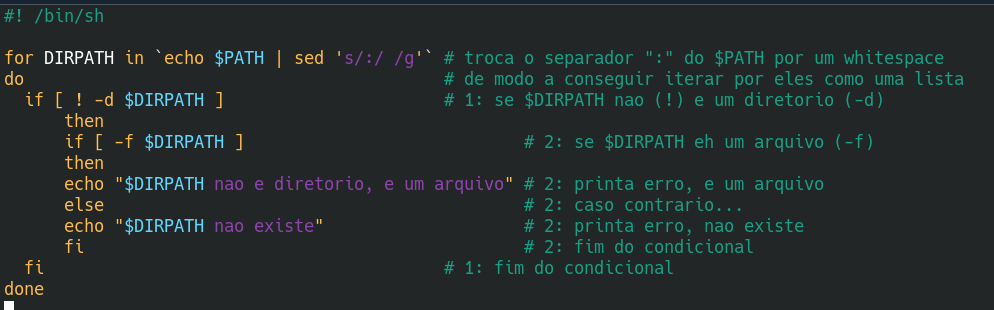
\includegraphics[width=\textwidth]{images/q5_c.png}
        \caption{Item (c)}
    \end{center}
\end{figure}

\begin{figure}[!ht]
    \begin{center}
        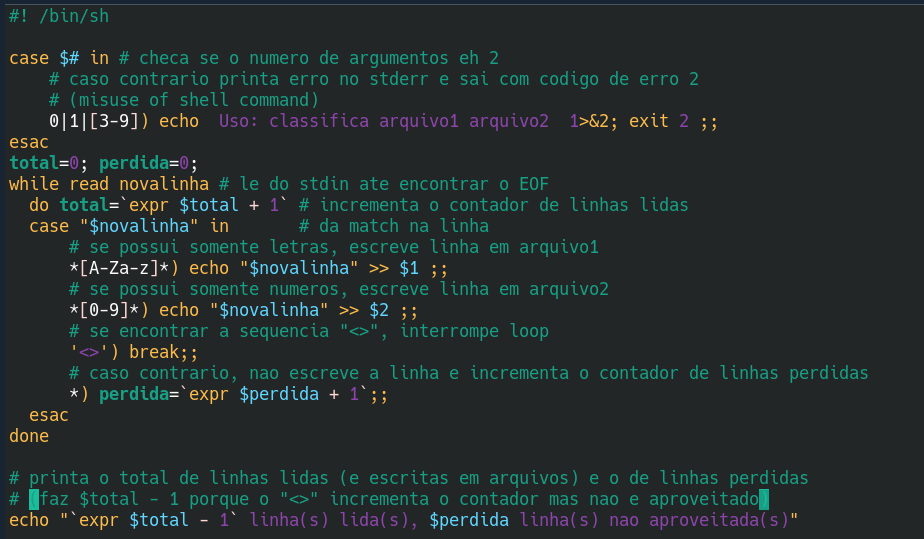
\includegraphics[width=\textwidth]{images/q5_d.png}
        \caption{Item (d)}
    \end{center}
\end{figure}

\section*{Questão 6}

O programa registra \textit{signal handlers} para os sinais \texttt{SIGTERM} e \texttt{SIGINT}, depois procede a entrar em \textit{idle} e checar a cada 5 segundos se recebeu um \textit{signal} do sistema, imprimindo uma mensagem quando detectar o recebimento de um.

\begin{figure}[!ht]
    \begin{center}
        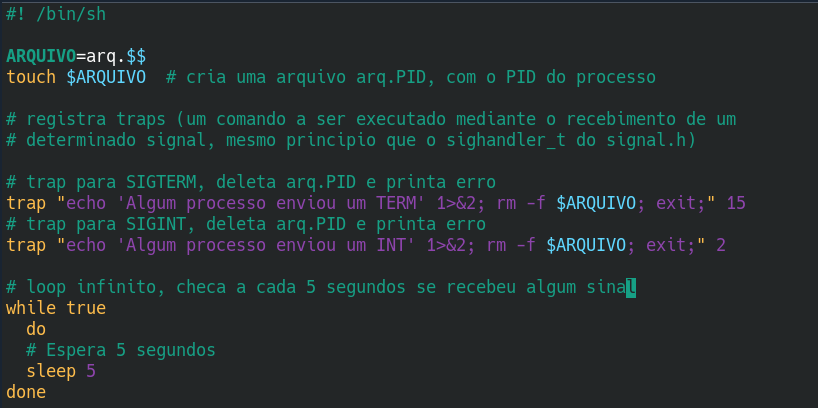
\includegraphics[width=\textwidth]{images/q6_comentario.png}
        \caption{Explicação detalhada do script \texttt{traps}}
    \end{center}
\end{figure}

\begin{figure}[!ht]
    \begin{center}
        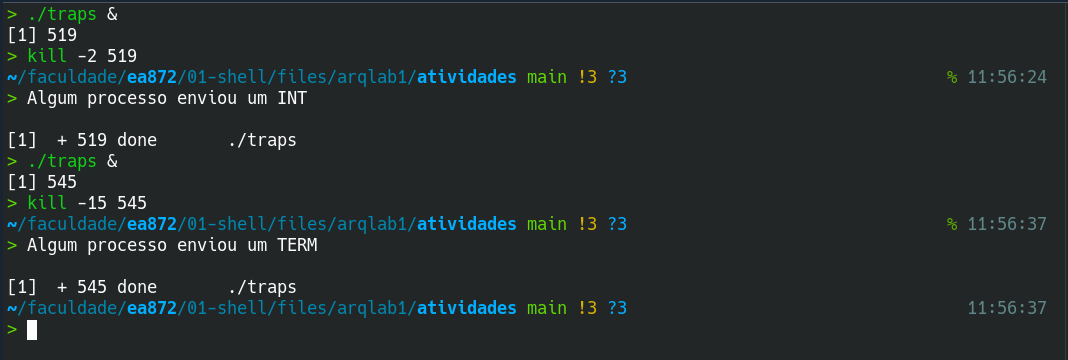
\includegraphics[width=\textwidth]{images/q6_execucao.png}
        \caption{Execução do script \texttt{traps}}
    \end{center}
\end{figure}

\newpage
\section*{Questão 7}

\begin{figure}[!ht]
    \begin{center}
        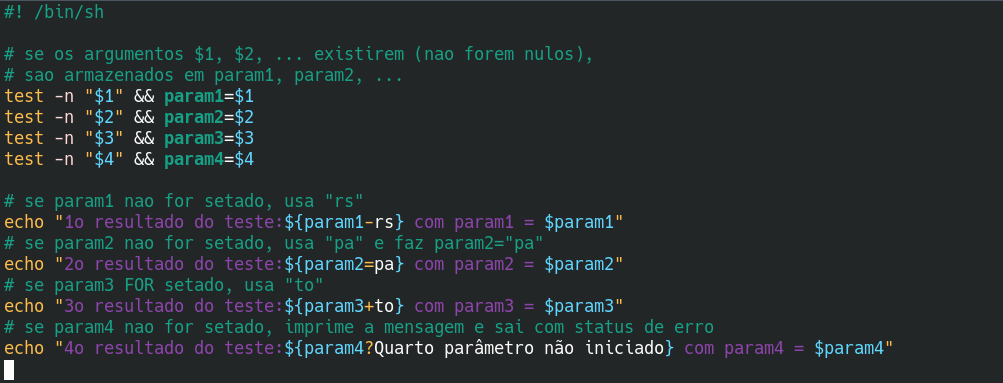
\includegraphics[width=\textwidth]{images/q7.png}
        \caption{Explicação detalhada do script \texttt{subspar}}
        \label{fig:q7}
    \end{center}
\end{figure}

\begin{figure}[!ht]
    \begin{center}
        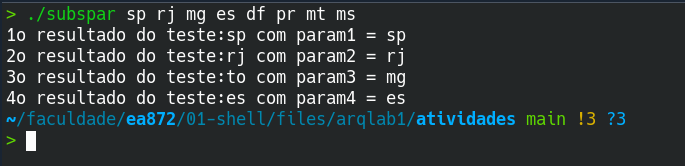
\includegraphics[width=\textwidth]{images/q7_execucao.png}
        \caption{Execução do script \texttt{subspar}}
        \label{fig:q7_exec}
    \end{center}
\end{figure}

A Figura \ref*{fig:q7} contém uma explicação passo a passo do script \texttt{subpar}. A Figura \ref*{fig:q7_exec} contém a execução do script com as entradas dadas. Percebe-se que as entradas \texttt{param1}, \texttt{param2} e \texttt{param4} se mantiveram inalteradas (porque estava setadas), enquanto \texttt{param3} foi impresso como \texttt{to} porque \texttt{param3} estava setado.

\newpage
\section*{Questão 8}

\begin{figure}[!ht]
    \begin{center}
        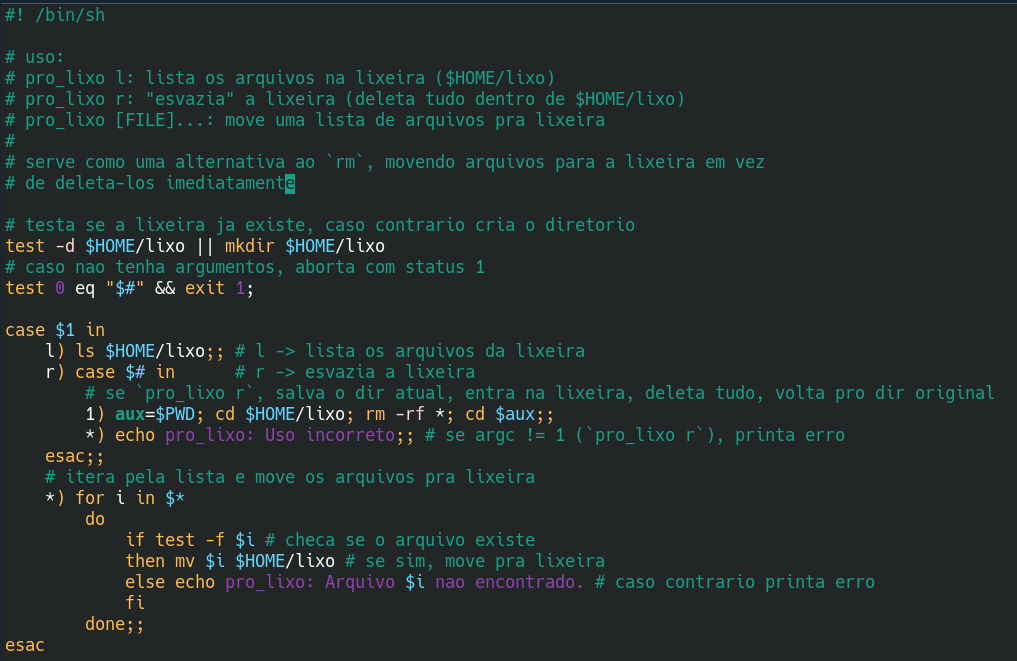
\includegraphics[width=\textwidth]{images/q8.png}
        \caption{Explicação detalhada do script \texttt{pro\_lixo}}
        \label{fig:q8}
    \end{center}
\end{figure}

Como detalhado na Figura \ref*{fig:q8}, a utilidade prática do script é mover arquivos para a lixeira (uma pasta localizada em \texttt{\$HOME/lixo}).

\newpage
\section*{Questão 9}

O script é basicamente uma implementação simplificada do comando \texttt{tree}, que imprime os arquivos dentro de uma pasta no formato de uma árvore. Abaixo seguem comentários detalhados do script (fiz uma pequena modificação para fazer ele funcionar sem estar no \texttt{\$PATH}, de modo a conseguir fazer rodar) e também uma imagem mostrando seu funcionamento:

\begin{figure}[!ht]
    \begin{center}
        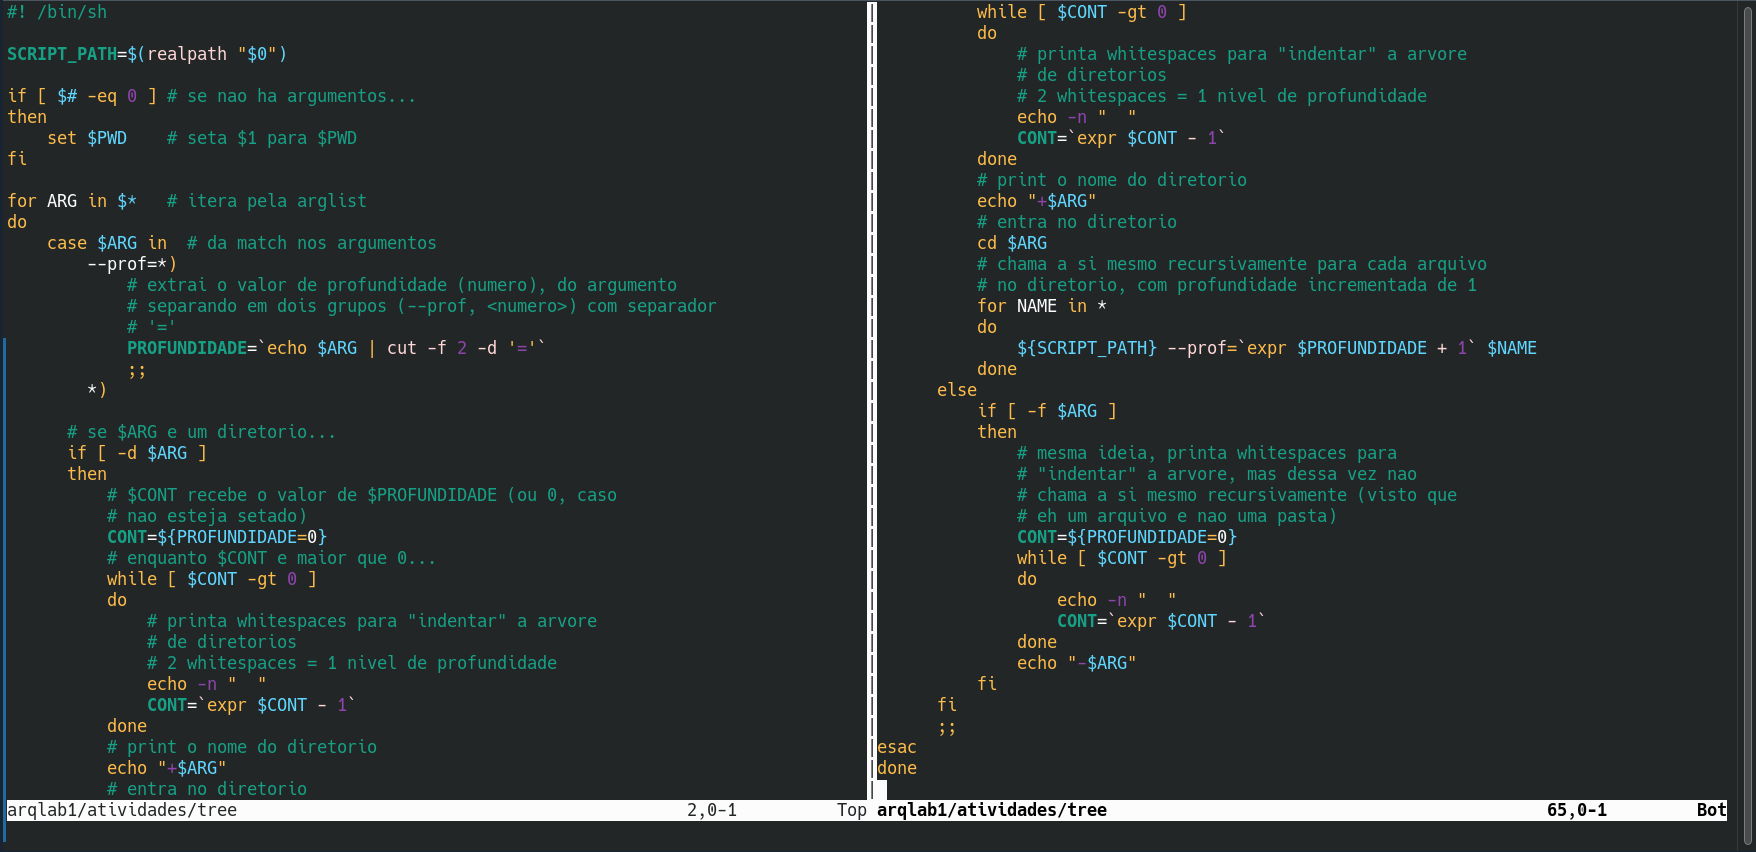
\includegraphics[width=\textwidth]{images/q9.png}
        \caption{Explicação detalhada do script \texttt{tree}}
    \end{center}
\end{figure}

\begin{figure}[!ht]
    \begin{center}
        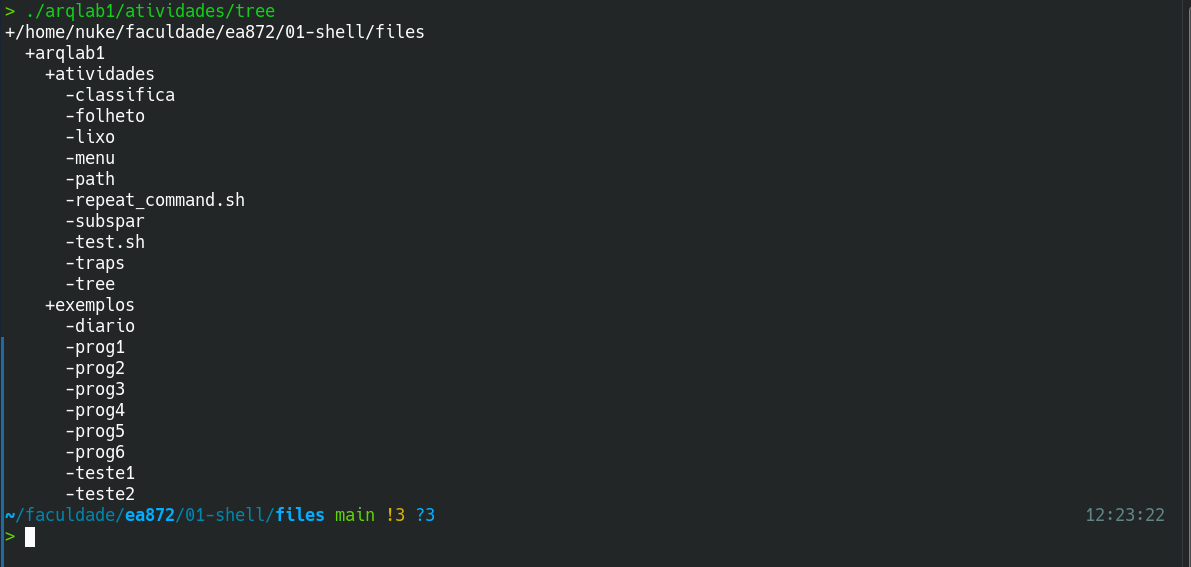
\includegraphics[width=\textwidth]{images/q9_exec.png}
        \caption{Execução do script \texttt{tree}}
    \end{center}
\end{figure}

\section*{Questão 10}

O script está em anexo junto a este relatório. Abaixo há uma imagem ilustrando o seu funcionamento:

\begin{figure}[!ht]
    \begin{center}
        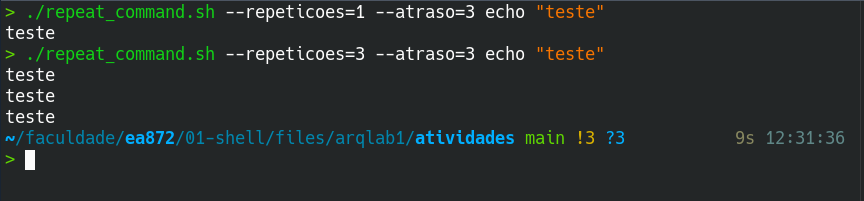
\includegraphics[width=\textwidth]{images/q10_exec.png}
        \caption{Execução do script \texttt{repeat\_command}. Observe a duração de 9s (3 execuções * delay de 3s).}
    \end{center}
\end{figure}

\section*{Questão 11}

Esse script também está em anexo junto ao relatório, e abaixo segue uma imagem dele em funcionamento:

\begin{figure}[!ht]
    \begin{center}
        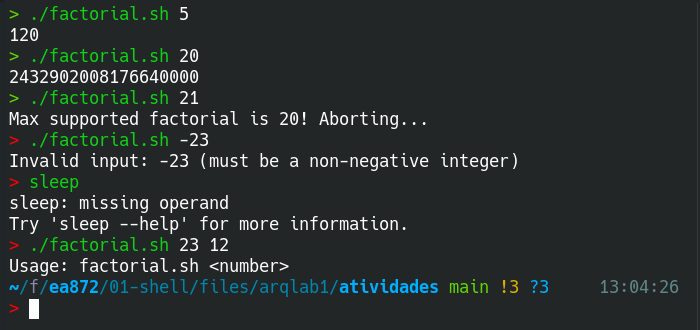
\includegraphics[width=\textwidth]{images/q11_exec.png}
        \caption{Execução do script \texttt{factorial.sh}}
    \end{center}
\end{figure}

\end{document}
